\documentclass{article}
\usepackage{graphicx} % Required for inserting images

\title{Chapter 1 (About the Manual/Notes?)}
\author{Daksh Pandey}
\date{February 2025}

\begin{document}

\maketitle

\section{Introduction}
First, the Intel has given a list of its processors for which the manuals' information hold true. I won't bother listing them again. Then comes the overview of the first volume. Again I wont bother listing the whole contents again and briefly describe them, just go over the manual yourself for that. 


\section{Notational Conventions}
Some basic terminologies which will only make reading further notes and manual easier. 
\subsection{Bit and Byte Order}
\begin{itemize}
    \item In the figure below, the lowest address is at the bottom right corner. 
    \item Highest address in at the upper left corner. 
    \item Numerical value of a set bit is equal to two raised to the power of the bit position. Bit positions are numbered from right to left. 
    \item Example: given the number 82, which in binary is 01010010, so the right-most 0 is at the 0th position and left-most 0 is at 7th position.
\end{itemize}
\begin{figure}
    \centering
    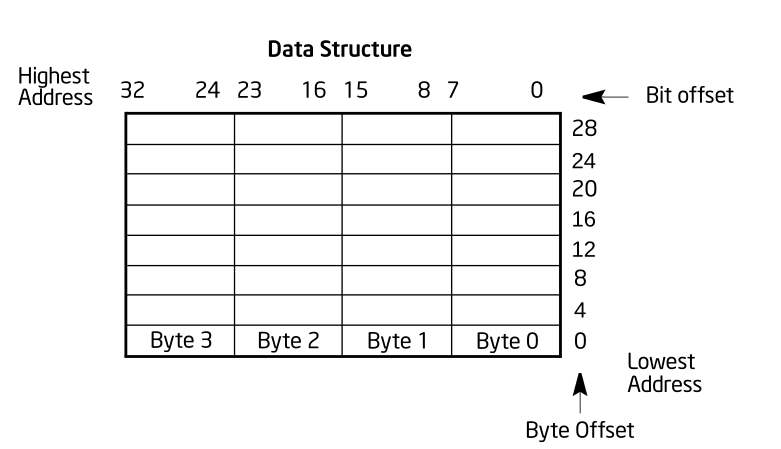
\includegraphics[width=1\linewidth]{Screenshot from 2025-02-07 16-36-12.png}
    \caption{Bit and Byte Order}
    \label{fig:bit_byte}
\end{figure}

\subsection{Reserved Bits and Software Compatibility}
\begin{itemize}
    \item Just don't depend on these bits. 
    \item These are essential for compatibility with the future processors. 
    \item These are not reliable, so just avoid using them.
\end{itemize}

\subsection{Instruction Operand}
\begin{itemize}
    \item When we use symbolic representation for instructions, some elements from IA-32 (Intel Architecture 32) AL is used. 
    \item According to IA-32's AL, instruction has the following format: 
    \begin{center}
        label: mnemonic arg1, arg2, arg3
    \end{center}
    \item \textbf{Label: }identifier followed by colon.
    \item \textbf{Mnemonic: }reserved name for a class of instruction opcodes. 
    \item Arguments are the operands. There may be 0 to 3 arguments, depending on the opcode. When presented, they may take form of literals or identifiers for data items. Operand identifiers are either reserved names of registers or assumed to be assigned to data items declared somewhere else. 

    \item When two operands in arithmetic or logical instruction, right is the source and left is the destination. 

    \item Example (from the manual only): 
    \begin{center}
        LOADREG: MOV EAX, SUBTOTAL
    \end{center}
    \item LOADREG is the label, MOV is mnemonic id of an opcode, EAX is the destination, SUBTOTAL is the source operand. 

    \item If you are wondering what Opcode is, it is a single instruction which can be executed by the CPU, MOV is an opcode (obviously in its mnemonic form). 
\end{itemize}


\subsection{Binary and Hexadecimal}
Cmon, you know these. Binary can sometimes be followed by B btw.

\subsection{Segmented Addressing}
\begin{itemize}
    \item Processor used byte addressing. 
    \item Other words, memory is organized and accessed as a sequence of bytes. 
    \item A byte address is always used, whether we are accessing only a byte or bytes.
    \item For future reference: word = 2 bytes, doubleword = 4 bytes, quadword = 8 bytes. 
    \item Range of memory that can be accessed: \textbf{address space}.
    \item Independent address spaces are called: \textbf{segments}.
    \item For example: 
    \begin{center}
        DS:FF79H
    \end{center}
    \item In the above example, DS it the segment and FF79H is the address whithin the segment. 
    \item Example below represents an instruction in the code segment. CS register points to the code segment and EIP register contains the address of instructions: 
    \begin{center}
        CS:EIP
    \end{center}
\end{itemize}

\subsection{Execption}
\begin{itemize}
    \item Event which occurs when an instruction causes an error. Example, attempt to divide by 0. 
    \item Some types of exceptions provide an error code. Sometimes we may not get an accurate reported code.
\end{itemize}


\textbf{All the image credits go to the reference at the end}
\begin{thebibliography}{9}
\bibitem{texbook}
Intel® 64 and IA-32 Architectures Software Developer’s Manual Volume-1\end{thebibliography}



\end{document}
